\documentclass[11pt,a4paper]{article}

% Fundamental packages
\usepackage[utf8]{inputenc}
\usepackage[T1]{fontenc}
\usepackage[english]{babel}
\usepackage{amsmath, amssymb, amsthm}
\usepackage{geometry}
\usepackage{graphicx}
\usepackage{booktabs}
\usepackage{hyperref}
\usepackage{xcolor}
\usepackage{fancyhdr}

% Page setup
\geometry{left=2.5cm, right=2.5cm, top=2.5cm, bottom=2.5cm}
\pagestyle{fancy}
\fancyhf{}
\rhead{\textit{Monte Carlo Simulation \& Variance Reduction}}
\lhead{\textit{Quantitative Research Note}}
\cfoot{\thepage}

% Mathematical environments
\newtheorem{theorem}{Theorem}
\newtheorem{proposition}{Proposition}
\newtheorem{definition}{Definition}
\newtheorem{remark}{Remark}

% Custom commands
\newcommand{\R}{\mathbb{R}}
\newcommand{\E}{\mathbb{E}}
\newcommand{\Q}{\mathbb{Q}}
\newcommand{\Prob}{\mathbb{P}}
\newcommand{\Var}{\mathbb{V}\text{ar}}
\newcommand{\Cov}{\mathbb{C}\text{ov}}
\newcommand{\F}{\mathcal{F}}

\title{\textbf{Pricing Arithmetic Asian Options via Monte Carlo Simulation and Control Variate Variance Reduction}}
\author{Amine El Mir \\ \small \textit{Department of Mathematics \& Data Science}}
\date{\today}

\begin{document}

\maketitle

\begin{abstract}
This paper presents a mathematical and numerical framework for pricing discrete arithmetic Asian options within the Black-Scholes-Merton model. Due to the absence of a closed-form analytical distribution for the arithmetic average of a geometric Brownian motion, we implement a standard Monte Carlo estimator and evaluate two convergence acceleration techniques under equal computational budgets: antithetic variates and a control variate method leveraging the exact analytical solution of the discrete geometric Asian option. Using an out-of-sample pilot scheme to eliminate finite-sample bias and validating against the Turnbull-Wakeman moment-matching approximation, numerical experiments demonstrate a variance reduction factor of $634.5\times$ and a net CPU time-adjusted efficiency gain exceeding $430\times$.
\end{abstract}

\section{Probabilistic Framework and Underlying Asset Dynamics}

Let $(\Omega, \F, (\F_t)_{t \in [0,T]}, \Prob)$ be a filtered probability space satisfying the usual conditions, where $(\F_t)_{t \in [0,T]}$ is the natural filtration generated by a standard one-dimensional Brownian motion $(W_t)_{t \in [0,T]}$.

By Girsanov's theorem and the completeness of the Black-Scholes market (Second Fundamental Theorem of Asset Pricing), there exists a unique equivalent martingale measure $\Q$ under which the discounted price process is a martingale. Under $\Q$, the dynamics of the non-dividend-paying underlying asset $(S_t)_{t \in [0,T]}$ are governed by the linear stochastic differential equation (SDE):
\begin{equation}
    dS_t = r S_t \, dt + \sigma S_t \, dW_t^\Q, \quad S_0 > 0
\end{equation}
where $r \in \R$ denotes the constant continuous risk-free interest rate, $\sigma > 0$ is the constant volatility, and $(W_t^\Q)_{t \in [0,T]}$ is a standard $\Q$-Brownian motion.

\begin{proposition}[Strong Solution and Exact Discretization]
Because the drift and diffusion coefficients satisfy global Lipschitz and linear growth conditions, the SDE admits a unique strong solution. Applying Itô's Lemma to $f(x) = \ln(x)$ yields the explicit form for all $t \in [0,T]$:
\begin{equation}
    S_t = S_0 \exp\left( \left(r - \frac{\sigma^2}{2}\right)t + \sigma W_t^\Q \right)
\end{equation}
Over a uniform monitoring grid $0 = t_0 < t_1 < \dots < t_m = T$ with time step $\Delta t = T/m$, the exact transition law satisfies the recursive scheme:
\begin{equation}
    S_{t_{j}} = S_{t_{j-1}} \exp\left( \left(r - \frac{\sigma^2}{2}\right)\Delta t + \sigma \sqrt{\Delta t} Z_j \right), \quad \text{where } (Z_j)_{1 \le j \le m} \underset{\text{i.i.d.}}{\sim} \mathcal{N}(0,1)
\end{equation}
\end{proposition}

\section{Asian Options and the Valuation Problem}

Unlike standard European vanilla options, the payoff of an Asian option depends on the average price of the underlying asset over the monitoring period $[0,T]$. This path-dependent averaging reduces sensitivity to spot price manipulation near maturity and yields a lower effective volatility than the underlying asset itself, making the Asian option less expensive than its European counterpart.

\begin{definition}[Discrete Arithmetic Asian Call]
Given a monitoring grid $(t_1, \dots, t_m)$, the terminal payoff at maturity $T$ of a discrete arithmetic Asian Call with strike $K > 0$ is defined as:
\begin{equation}
    H_A = (A_T - K)_+ = \max\left( \frac{1}{m} \sum_{j=1}^m S_{t_j} - K, \, 0 \right)
\end{equation}
The arbitrage-free price at $t=0$ is the discounted expectation under $\Q$:
\begin{equation}
    C_A = e^{-rT} \E^\Q\left[ (A_T - K)_+ \right]
\end{equation}
\end{definition}

Since a sum of log-normal random variables does not follow a known closed-form distribution, $C_A$ cannot be evaluated analytically. Conversely, the discrete geometric average preserves log-normality.

\begin{proposition}[Closed-Form Solution for the Discrete Geometric Asian Call]
Let $G_T = \left( \prod_{j=1}^m S_{t_j} \right)^{\frac{1}{m}}$ denote the discrete geometric average. The arbitrage-free price at $t=0$ of the geometric Asian Call, $C_G = e^{-rT} \E^\Q[(G_T - K)_+]$, admits an exact analytical formula:
\begin{equation}
    C_G = e^{-rT} \left( S_0 e^{\widetilde{r} T} \Phi(d_1) - K \Phi(d_2) \right)
\end{equation}
where $\Phi$ is the standard normal cumulative distribution function, and the effective discrete parameters are given by:
\begin{align*}
    \widetilde{\sigma} &= \sigma \sqrt{\frac{(m+1)(2m+1)}{6m^2}}, \quad & \widetilde{r} &= \left(r - \frac{\sigma^2}{2}\right)\frac{m+1}{2m} + \frac{\widetilde{\sigma}^2}{2} \\
    d_1 &= \frac{\ln(S_0/K) + (\widetilde{r} + \frac{1}{2}\widetilde{\sigma}^2)T}{\widetilde{\sigma}\sqrt{T}}, \quad & d_2 &= d_1 - \widetilde{\sigma}\sqrt{T}
\end{align*}
\end{proposition}

\begin{proof}
Expanding the log-geometric average yields:
\[
\ln\left(\frac{G_T}{S_0}\right) = \frac{1}{m} \sum_{j=1}^m \ln\left(\frac{S_{t_j}}{S_0}\right) = \left(r - \frac{\sigma^2}{2}\right) \frac{1}{m}\sum_{j=1}^m t_j + \frac{\sigma}{m} \sum_{j=1}^m W_{t_j}^\Q
\]
Since $t_j = j \frac{T}{m}$, the deterministic time average simplifies to $\frac{T}{m^2} \frac{m(m+1)}{2} = T \frac{m+1}{2m}$. Expressing $W_{t_j}^\Q = \sum_{k=1}^j (W_{t_k}^\Q - W_{t_{k-1}}^\Q)$ allows us to rewrite the Brownian sum in terms of independent increments:
\[
\frac{\sigma}{m} \sum_{j=1}^m W_{t_j}^\Q = \frac{\sigma}{m} \sum_{k=1}^m (m - k + 1) (W_{t_k}^\Q - W_{t_{k-1}}^\Q)
\]
By the independence and stationarity of Brownian increments, this linear combination is normally distributed with zero mean and variance:
\[
\frac{\sigma^2}{m^2} \frac{T}{m} \sum_{u=1}^m u^2 = \sigma^2 T \frac{m(m+1)(2m+1)}{6m^3} = \widetilde{\sigma}^2 T
\]
Hence, $\ln(G_T/S_0) \sim \mathcal{N}\left( (\widetilde{r} - \frac{1}{2}\widetilde{\sigma}^2)T, \, \widetilde{\sigma}^2 T \right)$, reducing the expectation to a Black-Scholes-type valuation with effective drift $\widetilde{r}$ and volatility $\widetilde{\sigma}$.
\end{proof}

\section{Monte Carlo Estimators and Variance Reduction}

\subsection{Standard Estimator and Convergence Rate}
Let $(Y^{(i)})_{1 \le i \le N}$ be i.i.d. replications of the discounted arithmetic payoff $Y = e^{-rT}(A_T - K)_+$. By the Strong Law of Large Numbers, the sample mean $\hat{C}_N^{\text{MC}} = \frac{1}{N} \sum_{i=1}^N Y^{(i)}$ converges almost surely to $C_A$. By the Central Limit Theorem (given $\Var(Y) = \sigma_Y^2 < +\infty$):
\begin{equation}
    \sqrt{N} \left( \hat{C}_N^{\text{MC}} - C_A \right) \underset{N \to +\infty}{\overset{\mathcal{L}}{\longrightarrow}} \mathcal{N}(0, \sigma_Y^2)
\end{equation}
The standard error decays at rate $\mathcal{O}(N^{-1/2})$.

\subsection{Antithetic Variates at Equal Computational Budget}
By symmetry of the standard normal distribution, if $Z = (Z_1, \dots, Z_m) \sim \mathcal{N}(0, I_m)$, then $-Z \sim \mathcal{N}(0, I_m)$. To ensure a fair comparison at an equal computational budget of $N$ total path evaluations (assuming $N$ is even), we generate $N/2$ independent pairs:
\begin{equation}
    \hat{C}_{N/2}^{\text{Anti}} = \frac{1}{N/2} \sum_{i=1}^{N/2} \frac{Y(Z^{(i)}) + Y(-Z^{(i)})}{2}
\end{equation}
Because the payoff mapping $Z \mapsto Y(Z)$ is coordinate-wise non-decreasing and $Z \mapsto Y(-Z)$ is coordinate-wise non-increasing in the independent Gaussian shocks $Z_j$, Harris's inequality (multivariate Chebyshev association inequality) guarantees that $\Cov(Y(Z), Y(-Z)) \le 0$. Consequently, the variance at equal computational cost satisfies:
\begin{equation}
    \Var\left(\hat{C}_{N/2}^{\text{Anti}}\right) = \frac{\Var(Y)}{N} \left( 1 + \rho_{Y(Z), Y(-Z)} \right) \le \Var\left(\hat{C}_N^{\text{MC}}\right)
\end{equation}

\subsection{Control Variate Method and Pilot Estimation}
We exploit the strong collinearity between the discounted arithmetic payoff $Y = e^{-rT}(A_T - K)_+$ and the discounted geometric payoff $X = e^{-rT}(G_T - K)_+$, whose exact expectation $\E^\Q[X] = C_G$ is known from Proposition 2.

For any fixed coefficient $\beta \in \R$, the control variate estimator is defined as:
\begin{equation}
    \hat{C}_N^{\text{CV}}(\beta) = \frac{1}{N} \sum_{i=1}^N \left( Y^{(i)} - \beta \left( X^{(i)} - C_G \right) \right) = \bar{Y}_N - \beta \left( \bar{X}_N - C_G \right)
\end{equation}

\begin{proposition}[Optimal Control Variate]
For any deterministic $\beta \in \R$, $\hat{C}_N^{\text{CV}}(\beta)$ is an unbiased estimator of $C_A$. Its variance is uniquely minimized at:
\begin{equation}
    \beta^* = \frac{\Cov(X,Y)}{\Var(X)}
\end{equation}
yielding a theoretical variance reduction ratio of:
\begin{equation}
    \frac{\Var\left(\hat{C}_N^{\text{CV}}(\beta^*)\right)}{\Var\left(\hat{C}_N^{\text{MC}}\right)} = 1 - \rho_{X,Y}^2
\end{equation}
where $\rho_{X,Y} \in [-1,1]$ denotes the Pearson correlation coefficient between $X$ and $Y$.
\end{proposition}

\begin{proof}
By linearity of expectation, $\E^\Q[\hat{C}_N^{\text{CV}}(\beta)] = \E^\Q[Y] - \beta(\E^\Q[X] - C_G) = C_A$. The single-path variance $g(\beta) = \Var(Y - \beta X) = \Var(Y) - 2\beta\Cov(X,Y) + \beta^2\Var(X)$ is strictly convex in $\beta$ since $\Var(X) > 0$, attaining its global minimum at $g'(\beta^*) = 0 \iff \beta^* = \frac{\Cov(X,Y)}{\Var(X)}$. Substituting $\beta^*$ gives $\Var(Y - \beta^* X) = \Var(Y)(1 - \rho_{X,Y}^2)$.
\end{proof}

\begin{remark}[Out-of-Sample Pilot Estimation]
In practice, $\beta^*$ is unknown. Estimating $\hat{\beta}^*$ and evaluating $\hat{C}_N^{\text{CV}}$ on the same sample introduces a finite-sample bias of order $\mathcal{O}(1/N)$ due to the dependence between $\hat{\beta}^*$ and $\bar{X}_N$. To preserve strict unbiasedness, we estimate $\hat{\beta}^*$ on an independent pilot run of size $N_{\text{pilot}} = 10,000$ before evaluating the estimator out-of-sample on the $N = 100,000$ primary trajectories. The standard error of $\hat{C}_N^{\text{CV}}$ is then computed directly from the empirical standard deviation of the controlled observations $Y^{(i)} - \hat{\beta}^* X^{(i)}$.
\end{remark}

\section{Model Validation and Numerical Results}

Simulations are executed in Python (\texttt{NumPy} default random generator \texttt{PCG64}, fixed seed \texttt{42} for exact reproducibility) under the market parameters: $S_0 = 100$, $K = 100$, $r = 0.05$, $\sigma = 0.20$, $T = 1.0$ year, and $m = 252$ daily steps.

\subsection{Validation Checks and Analytical Benchmarks}
\begin{enumerate}
    \item \textbf{Boundary Consistency ($m=1$):} For a single monitoring date $m=1$, both the arithmetic and geometric Asian options collapse to a standard European Call. We verify numerically that $C_G(m=1) = 10.450584$, matching the exact Black-Scholes price to machine precision ($10^{-15}$), and yielding zero variance for the control variate estimator.
    \item \textbf{Discrete Geometric Benchmark ($m=252$):} Using Proposition 2, the discrete effective parameters are $\widetilde{\sigma} = 0.11581$, $\widetilde{r} = 0.02177$, $d_1 = 0.2458$, and $d_2 = 0.1300$, yielding an exact discrete geometric Call price of $\mathbf{C_G = 5.5664}$ (as opposed to $5.5468$ in the continuous $m \to \infty$ limit).
    \item \textbf{Turnbull-Wakeman Approximation:} Matching the exact first two moments of the discrete arithmetic average ($M_1 = \E^\Q[A_T]$ and $M_2 = \E^\Q[A_T^2]$) to a log-normal distribution provides an independent analytical benchmark of $\mathbf{C_{\text{TW}} = 5.7850}$.
\end{enumerate}

\subsection{Empirical Performance Comparison}
The independent pilot run ($N_{\text{pilot}} = 10,000$) yields $\hat{\beta}^* = 1.0414$. Across the $N = 100,000$ out-of-sample paths, the empirical correlation between $X$ and $Y$ is $\hat{\rho}_{X,Y} = 0.999212$, which matches the theoretical variance reduction factor $1 / (1 - \hat{\rho}_{X,Y}^2) = 634.5\times$.

\begin{table}[h!]
\centering
\caption{Estimator performance at equal budget ($N = 100,000$ total path evaluations)}
\vspace{0.2cm}
\resizebox{\textwidth}{!}{%
\begin{tabular}{@{}lcccccc@{}}
\toprule
\textbf{Estimation Method} & \textbf{Estimated Price} & \textbf{Standard Error} & \textbf{95\% Confidence Interval} & \textbf{Equal-Budget VRF} & \textbf{CPU Time (s)} & \textbf{Time-Adjusted Gain} \\ \midrule
Standard MC ($N$ paths) & $5.7888$ & $0.0254$ & $[5.7391, \, 5.8385]$ & $1.0 \times$ & $0.68\text{ s}$ & $1.0 \times$ \\
Antithetic ($N/2$ pairs) & $5.7924$ & $0.0178$ & $[5.7575, \, 5.8273]$ & $2.0 \times$ & $0.70\text{ s}$ & $2.0 \times$ \\
\textbf{Control Variate ($N$ paths)} & $\mathbf{5.7830}$ & $\mathbf{0.0010}$ & $\mathbf{[5.7810, \, 5.7850]}$ & $\mathbf{634.5 \times}$ & $\mathbf{0.99\text{ s}}$ & $\mathbf{435.8 \times}$ \\ \bottomrule
\end{tabular}%
}
\label{tab:results}
\end{table}

\begin{figure}[h!]
    \centering
    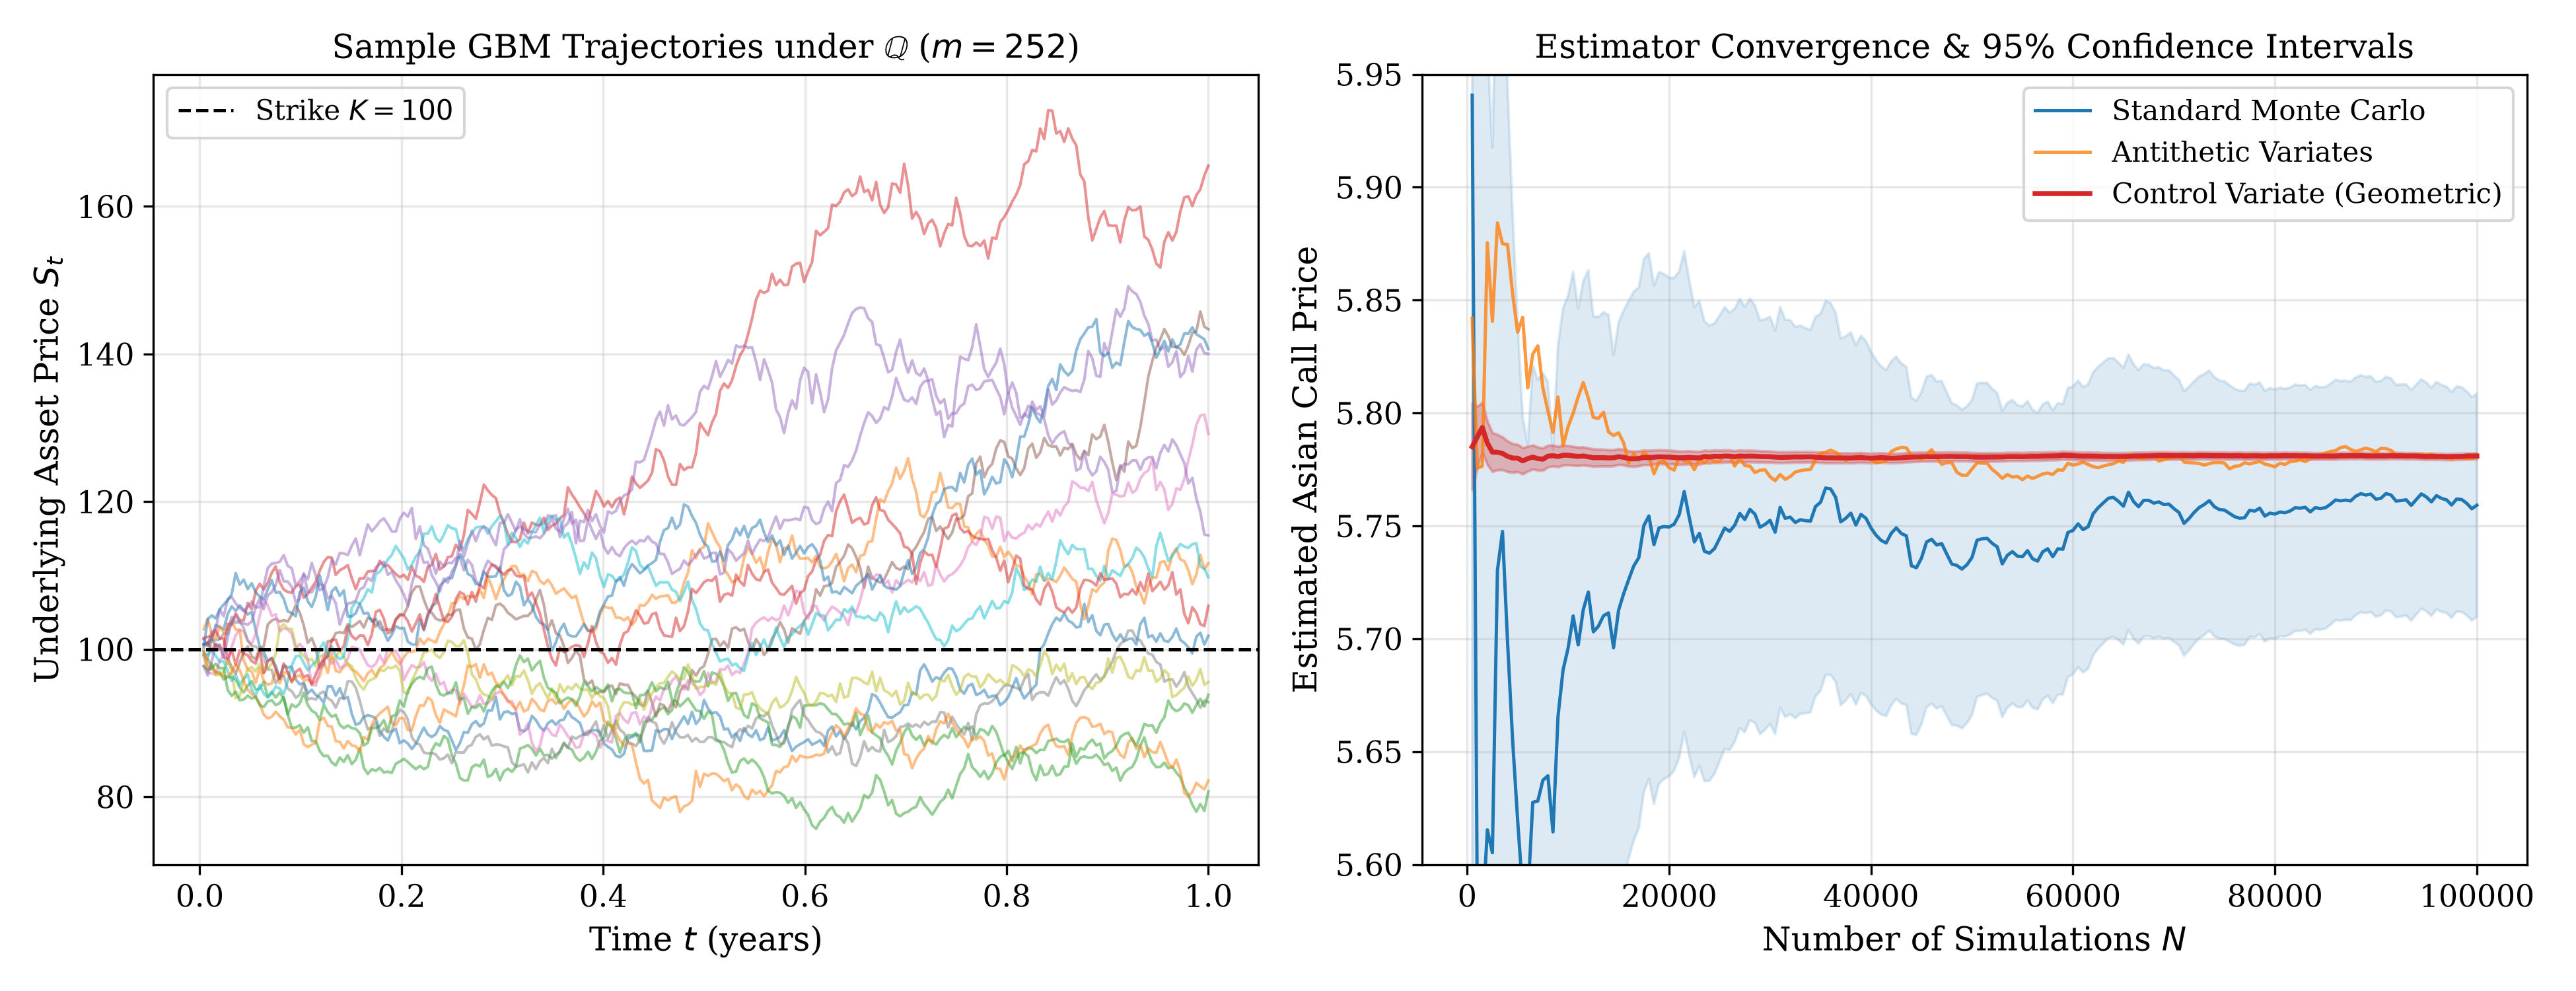
\includegraphics[width=0.95\textwidth]{convergence_mc.png}
    \caption{Left: Sample trajectories of the geometric Brownian motion under $\Q$. Right: Convergence of the three estimators as a function of total path evaluations $N$ towards the true price ($\approx 5.783$), illustrating the contraction of the 95\% confidence interval.}
    \label{fig:convergence}
\end{figure}

Table \ref{tab:results} and Figure \ref{fig:convergence} confirm full consistency across all estimators:
\begin{itemize}
    \item All three estimators converge consistently towards $5.7830$, in close agreement with the Turnbull-Wakeman analytical approximation ($5.7850$).
    \item At an equal computational budget of $100,000$ path evaluations, antithetic variates reduce variance by a factor of $2.0\times$.
    \item Accounting for the additional CPU overhead of the pilot run and geometric average evaluation ($0.99\text{ s}$ vs.\ $0.68\text{ s}$), the control variate method achieves a net time-adjusted efficiency gain of $435.8\times$.
\end{itemize}

\section{Conclusion}
This study illustrates how leveraging an exact closed-form solution of an auxiliary contract (the discrete geometric Asian Call) as a control variate overcomes the slow convergence of Monte Carlo simulation for path-dependent derivatives. Future extensions include combining antithetic sampling with multiple control variates (e.g., incorporating the terminal spot $S_T$), computing pathwise sensitivities (Delta $\Delta$, Vega $\mathcal{V}$), and extending the framework to stochastic volatility models.

\end{document}
